% Chapter 3 - Methodology

% \glsresetall % reset the glossary to expand acronyms again
\chapter[Distributed Deep Learning]{Distributed Deep Learning}\label{ch:DistributedDL}
\index{Distributed Deep Learning}
Over the past decade, machine learning, specifically deep learning (DL), has exploded in popularity.
Several incredibly challenging problems have recently been solved using emerging techniques, classic examples include computer vision \cite{Krizhevsky2012AlexNet}, and natural language processing \cite{Vaswani2017AttentionTransformer}.
Furthermore, more traditional scientific HPC fields like climate modelling \cite{Ham2019DLENSOForcasts} and cosmology \cite{Mathuriya2019Cosmoflow} are starting to adopt DL methods.
There is an incredible demand for DL as academia and industry rush to develop new models to solve more problems.
However, DL is incredibly computationally intensive, and depending on the number of model parameters and the dataset size, training time can span from hours to weeks.
To address these issues, DL practitioners are adopting HPC techniques to parallelize the training process at a massive scale and build larger models faster.
Parallelization strategies are diverse, but the three methods used at scale are hyperparameter search for evaluating different architectures, model parallelism to stretch a model across multiple nodes, and data parallelism to process numerous samples concurrently and lower time to convergence.
Data parallelism is the most well-understood parallelization strategy, having existed long before the recent AI revolution \cite{Zhang1990BPonCM2}.
It is relatively easy to deploy, has a well-understood communication pattern, and is highly scalable.

This chapter contains a high-level overview of current distributed DL practices focusing on data-parallel strategies.
We then outline the state-of-the-art tools used at scale and investigate HPC methods that have accelerated data-parallel training in literature.

\section{Deep Learning}
Deep learning is a supervised learning technique where a model is trained to approximate some ground truth source, typically a dataset.
Formally, deep learning training tries to find a function $f: X\longrightarrow Y$ which maps data from sample space $X$ to label space $Y$.
To predict how accurate $f$ is for a sample $x$, we define a loss function $L_D(f)=\mathbb{P}[f(x)\neq h(x)]$, where $x$ is a sample in dataset $D$ with label $h(x)$.
In practice, $f$ will belong to a class of function $\mathcal{H}$ containing functions $f_w$, where $w$ is a vector of parameters.
To train a model, a training algorithm will try to find some value for $w$ which minimizes the loss function of $f$ over $D$, formally:
\begin{equation}
    \argmin_{w\in\mathcal{H}} L_D(f_w) = \argmin_{w\in\mathcal{H}} \mathbb{E}_{x\in D}[\ell (w,x)]
    \label{eq:argmin-loss}
\end{equation} 
Where $\ell:\mathcal{H}\times X\longrightarrow \mathbb{R}^+$ is the loss function for an individual sample. 

Many optimization algorithms can solve equation \ref{eq:argmin-loss}, but the most widely adopted algorithm is minibatch stochastic gradient descent (SGD).
Standard gradient descent relies on a continuous optimization space to intelligently sample points, but the datasets used in DL are not continuous.
SGD methods used in practice randomly sample points in the dataset, and while they do converge, they tend to take much longer than traditional gradient descent \cite{Robbins1951StochasticAproxmethod}.
Traditional SGD samples one data point at a time, but on modern hardware, we can increase device utilization, and throughput by grouping multiple data points using a batch method \cite{Le2011OnOptMethodsforDL}.
Batch methods sample a set of data points to assemble a batch, calculate an update step for each sample in the batch, and apply the average update of the batch to the model. 

\begin{algorithm}
    \caption{Minibatch SGD}
    \label{alg:MinibatchSGD}
    \begin{algorithmic}[1]
        \For {t = 0 \textbf{to} $\frac{|D|}{B}*epochs$} \Comment{for a specified number of iterations over the dataset}
        \State $\Bar{x}\leftarrow$ Vector of $B$ Random elements from $D$ \Comment{Take minibatch from dataset}
        \State $w_{mb}\leftarrow w^{(t)}$ \Comment{Load weights}
        \State $f\leftarrow \ell(w_{mb},\Bar{x},h(\Bar{x}))$ \Comment{Forward evaluation with minibatch}
        \State $g_{mb}\leftarrow \nabla \ell(w_{mb}, f)$ \Comment{Backpropogate to calculate gradient}
        \State $\Delta w \leftarrow u(g_{mb}, w^{(0,...,t)}, t)$ \Comment{Calculate weight update, performs allreduce}
        \State $w^{(t+1)}\leftarrow w_{mb} + \Delta w$ \Comment{Apply weight updates to next itteration}
        \EndFor
    \end{algorithmic}
\end{algorithm}

Algorithm \ref{alg:MinibatchSGD} provides a textbook example of a minibatch SGD algorithm.
The main loop of the algorithm iterates over the entire dataset in what's known as an epoch, this is often done a predefined number of times. 
Still, other stopping criteria can include an evaluation threshold on an external validation dataset or a collapse in the loss function.
A batch of data is sampled from the training dataset in line 2, the dataset is shuffled between epochs to generate different minibatches for each epoch.
The minibatch samples are propagated through the model in the forward pass on line 4, and the set of forward pass results is used to calculate a set of gradients in line 5. 
Line 6 uses an update function to calculate the weight updates, this function is responsible for combining the gradients of all the samples into weight updates to be applied to the next iteration of the model (line 7).

While this algorithm seems straightforward, the research space is massive, spanning from the model's architecture to tweaking parts of the training algorithm.
The optimization space can have multiple minimums, and deliberate steps must be taken to ensure the global minimum is found. 
Weight initialization is another issue since the final accuracy can be heavily influenced by $w^{(0)}$, initialization methods include random values, informed decisions, or transfer learning from other pre-trained models \cite{Glorot2010XavierInitalization}.
The weight update rule $u$ has also undergone a lot of research.
If update steps are too large, the model will not generalize and will be unstable, but training can take an exceedingly long time if updates are too small.
The most straightforward rule, $u_{sgd}(g)=-\eta \cdot g$, multiplies the gradient by a learning rate $\eta$, but the learning rate can be changed over time, with a common practice of exponentially shrinking the gradient with larger values of $t$.
More clever methods can include momentum, which uses the difference between current and past weights to influence update magnitude, and modern techniques, like Adam \cite{Kingma2015Adam}, leverage the first and second moments of the gradient to update learning rates individually for each weight in the model.

The model's architecture also plays an important role.
The founding idea for neural networks was to approximate the structure of neurons in the brain mathematically.
Individual neurons take a set of inputs, calculate a weighted sum across a set of weights, apply an activation function to introduce nonlinearity, and pass the output on to other neurons. 
Neurons are organized into layers, often structured in a fully connected manner where the output of one neuron is connected to every neuron in the next layer.
The model's width is defined by the number of neurons in a layer, while the number of layers defines the depth.
These early feed-forward networks have a powerful ability to learn non-linear relationships and can be efficiently implemented using general matrix-matrix multiplications (GEMM).
However, different layer types have been proposed which can extract specific features of different kinds of data; famous examples include convolutional layers for images \cite{Krizhevsky2012AlexNet}, recurrent layers for sequence data \cite{cho2014PhraseRepresentationRNN}, and transformer layers for text \cite{Vaswani2017AttentionTransformer}.
Further, many different activation functions can be used, with popular choices including sigmoid and rectified linear units \cite{Nair2010ReLU}.

However, one prevalent trend of DL (in fact, this is where the 'deep' in \textit{deep learning} comes from) is that larger models and larger datasets give better performance \cite{Kaplan2020ScalingLawsForNLModels, Ben-Nun2019DemystifyDL}.
There is a consistent trend of larger models training on larger datasets, however, the more these factors scale, so does the required training time.
To address these issues, several parallelization strategies have been applied.

Individual layer operations were the initial target for optimization. 
Many hardware providers have released software libraries designed to run layer-specific operations like convolutions and GEMM as fast as possible; examples include Intel's MKL and Nvidia's CUDNN \cite{MKL, cuDNN}. 
The compute-intensive nature of DL models has led to the wide adoption of GPUs as the massively parallel capabilities of these accelerators can blast through training and inference orders of magnitude faster than CPUs.
GPUs still have a limit to how many TFLOPs they can drive, and there are limits to the amount of accelerator memory, but both limitations can be broken by scaling across a cluster.

\section{Parallel Deep Learning}
Mapping DL training to a distributed memory environment creates several unique challenges.
The three most common strategies for parallelizing DL are hyperparameter search, where model architectures are evaluated concurrently; model parallelism, where a model's weights are distributed across resources; and data parallelism, which leverages parallelism in the training algorithm to concurrently evaluate samples in a batch.
Each method has its strength and targets a slightly different aspect of DL scaling while having its corresponding performance characteristics that must be accounted for.

\subsection{Hyperparameter search}
The features specifying a DL model can be lumped into two categories, parameters and hyperparameters.
Parameters are values filled by the optimization algorithm and is essentially synonymous with the model's weights. 
Conversely, hyperparameters focus on specifying the structure of the model and remain unchanged during training.
Hyperparameters include structural features of the model, like the number and types of layers, activation function, and loss function. 
They can also extend to the training algorithm with tunables like learning rate, learning rate decay, and batch size.
The setup has an outsized impact on model performance, so often, a lot of model development time goes into hyperparameter selection. 
However, each new hyperparameter adds another search dimension and exponentially increases the search space.
Therefore, automated hyperparameter search strategies are a popular target for parallelization at scale.

Research in hyperparameter search systems tends to investigate the search algorithm. 
Initially proposed search algorithms include sequential search heuristics, like grid search \cite{Hadjis2016Omnivore}, where a series of candidates are identified, models are trained for each, and the search space is iteratively refined based on the training results.
More clever techniques have used evolutionary algorithms \cite{Young2017EvolveNLWithHPC, Real2017LargeScaleEvolutionOfCV}, which generates a population of candidate models and iteratively removes underperforming models and replaces them with higher-performing models with random perturbations, or reinforcement learning \cite{Zoph2017NeuralArchSearchReinformceLearn} which uses gradient-based optimization to discover more optimal model architectures.

At its core, hyperparameter search trains a DL model (which can take tens of minutes to hours), validates the model's performance, and updates a search space (send and receive a few megabytes).
This makes hyperparameter search an incredibly compute-intensive task with little communication, making it a great candidate for parallelization.
Large-scale hyperparameter search systems are often based on a server/worker design, where the centralized server manages the search algorithm and issues models for worker nodes to train and evaluate.
These systems generate relatively little communication as model architectures can be specified in a few bytes, workers can take hours to train a model, and they have been relatively easy to scale to exceedingly large systems \cite{Young2017EvolveNLWithHPC}.

\subsection{Model Parallelism}
\begin{figure}
    \centering
    % 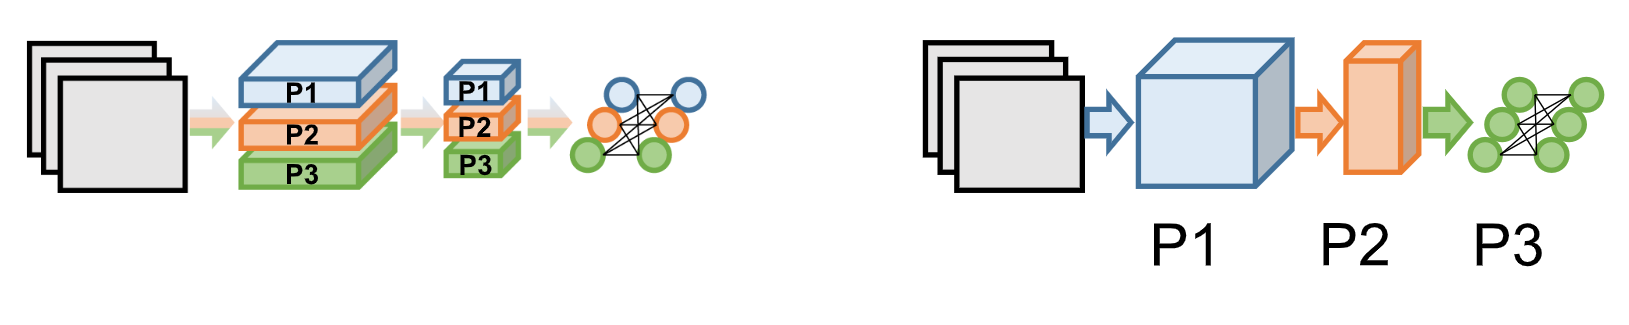
\includegraphics[width=15cm]{3_Chapters/3_Chapter_DistributedDL/Figs/model_parallel_decomposition.png}
    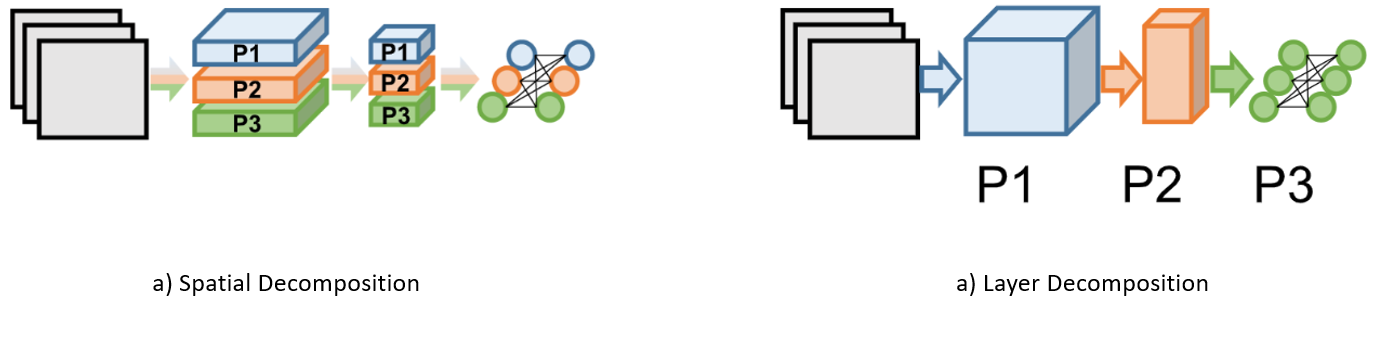
\includegraphics[width=15cm]{3_Chapters/3_Chapter_DistributedDL/Figs/model_parallel_decomposition_v2.png}
    \caption{Tow methods for partitioning a neural network, left is spacial decomposition, right is layer-wise.}
    \label{fig:model-parallel-decomposition}
\end{figure}

\begin{figure}
    \centering
    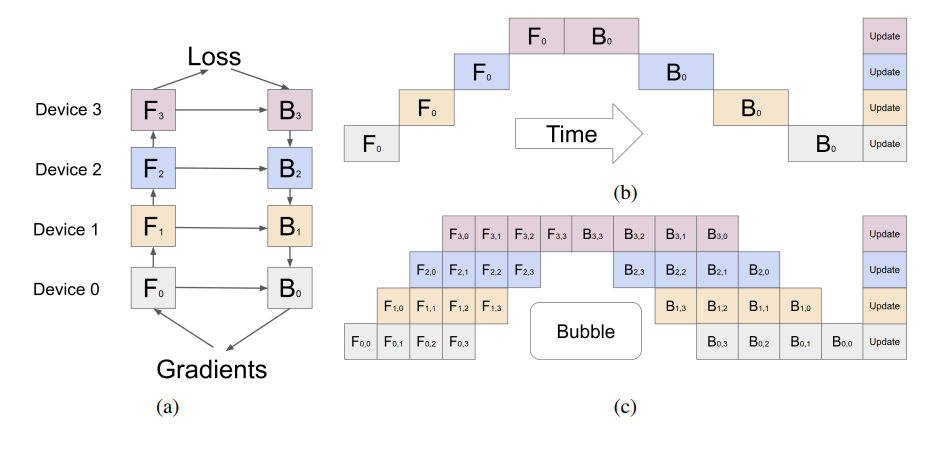
\includegraphics[width=15cm]{3_Chapters/3_Chapter_DistributedDL/Figs/layer_decomposition_bubble_gpipe.png}
    \caption{taken from \cite{Huang2019Gpipe}}
    \label{fig:layer_decomp_bubble}
\end{figure}

Model parallelism splits the model's architecture into chunks and distributes partitions across processing resources, the two basic decomposition patterns are given in figure \ref{fig:model-parallel-decomposition}
DL models can be decomposed across the depth in a layer-wise manner or decomposed spatially across the width,  
Layer-wise model parallelism uses individual layers as units for work and issues one or more layers on each processing resource \cite{Abadi2015TensorflowWhitepaper}. 
Spatial decomposition takes a finer-grained approach, it breaks individual layers into sections and can map a single layer across multiple ranks \cite{VanEssen2015LBANN}.
It is also possible for both strategies can be used in parallel, which provides flexibility to map network elements to compute to maximize machine utilization \cite{Dean2012DistBelif}.

The critical benefit of model parallelism is how it removes model size scaling limits.
The amount of available memory often limits the number of model parameters, but these techniques allow networks to access a larger memory pool. 
However, the added complexity of a distributed memory environment can add several complications to model design. 
Layer-wise decomposition can introduce 'bubbles' of idle time, as the forward pass must be complete before weight updates can be calculated, forcing ranks earlier in the network to stall as deeper ranks complete their work \cite{Huang2019Gpipe}.
The distribution of parameters leads to complicated communication patterns.
Spatial decomposition can generate several complicated communication patterns, these can vary from halo exchange to all-to-all collectives and are often dependant on the model's architecture \cite{Coates2013DLwithCOTSHPC, Dryden2019ImprvScaleofCNN}.
Furthermore, these drawbacks can compound when spatial and layer decomposition are combined, increasing the complexity needed in model parallel training systems.
For this reason, there is currently a lot of ongoing research in model-parallel training.

\subsection{Data paralleism}
\begin{figure}
    \centering
    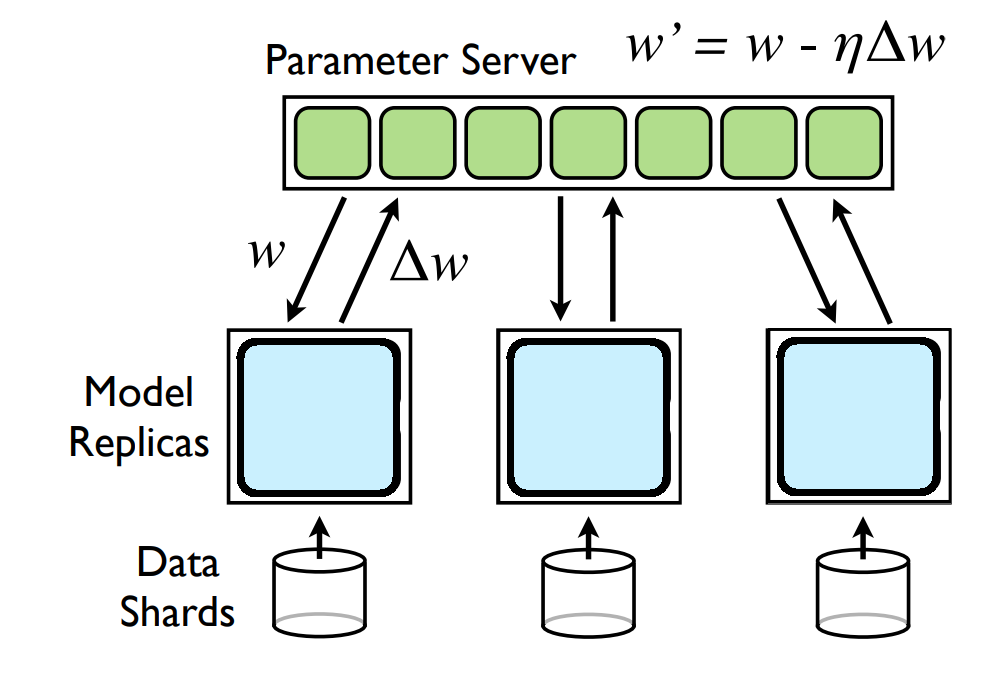
\includegraphics[width=10cm]{3_Chapters/3_Chapter_DistributedDL/Figs/parameter_server.png}
    \caption{Parameter server, taken from \cite{Dean2012DistBelif}}
    \label{fig:parameter-server}
\end{figure}

\begin{figure}
    \centering
    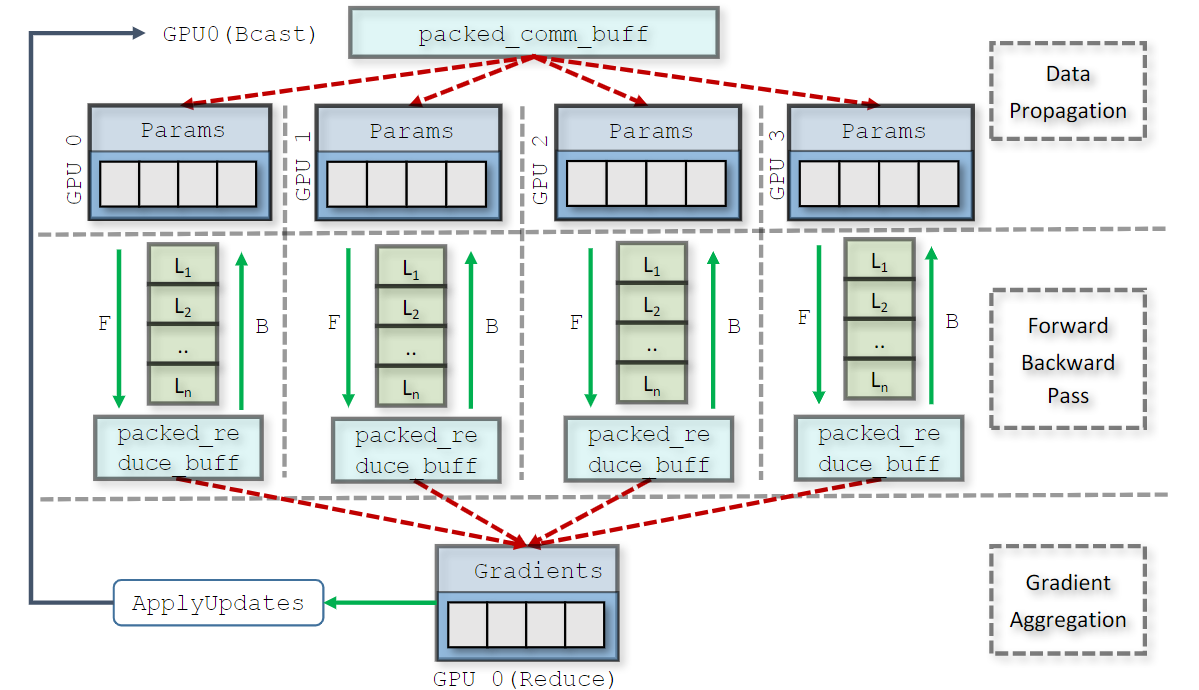
\includegraphics[width=15cm]{3_Chapters/3_Chapter_DistributedDL/Figs/Caffee_DP_arch.png}
    \caption{Data parallel architecture of Caffe, taken from \cite{Awan2017InDepthPerfCharOfDNN}}
    \label{fig:caffe-dp-arch}
\end{figure}

Recall that in minibatch SGD, samples within a batch are not computationally dependent on each other.
Data parallelism leverages this fact to evaluate multiple samples within a minibatch concurrently and speed up the time to convergence.
Each process performs a forward and backward pass on a subset of the minibatch and calculates a local weight update, and the global average of all weight updates is applied to the model for the next iteration.
However, there are mathematical challenges to scaling, adding more processes implicitly increases the batch size, which impacts the model's final convergence, and larger batch sizes tend to perform poorly \cite{Keskar2016LargeBatchTraining}.
To combat this, researchers have found that appropriately tuned update rules and regularization layers, like batch normalization, improve large batch training \cite{You2018ImgNetInMin, Goyal2017FacebookImgNet1Hour}. 

The other challenge is the added communication.
$\Delta w$ needs to be identical across all ranks, this adds synchronization and communication to every epoch and can become the scaling bottleneck.
The first forays into large-scale data-parallel deep learning were built around centralized parameter server \cite{Dean2012DistBelif, Chilimbi2014ProjectAdam}.
This architecture, outlined in figure \ref{fig:parameter-server}, designates a coordinator process to manage the global state of the model, and issue weights and minibatches to workers which calculate weight updates in parallel, then return their $\delta w$ to the server which updates the model for the next round.
This design is fault-tolerant, workers can drop out, and training can continue without hiccups. 
However, the fatal flaw of this design is how the server can become a communication choke point.
Using communication modelling established in Section \ref{sec:CH2-MPI-AlgStructure}, a singular server would need to receive $p$ messages and perform $p$ reductions, introducing a whopping cost of $p(\alpha+n(\beta+\gamma))$, the linear scaling w.r.t $p$ makes this architecture prohibitively expensive to run at scale.
There have been attempts to mitigate this issue using techniques like a hierarchical pool of parameter servers \cite{Gupta2016Rudra}.
However, the centralized nature of the system still adds a fundamental scaling limit.

\begin{figure}
    \centering
    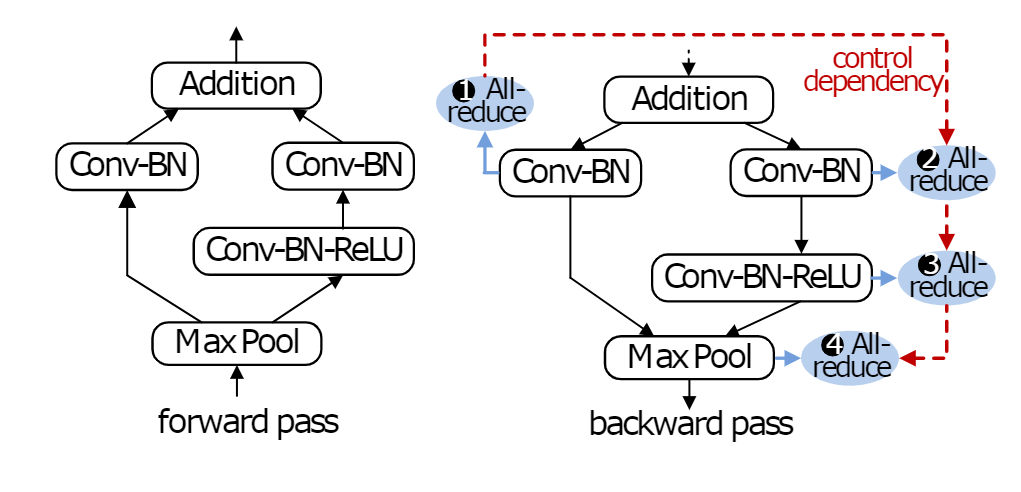
\includegraphics[width=15cm]{3_Chapters/3_Chapter_DistributedDL/Figs/ResNet_block_control_dependency.png}
    \caption{ResNet block, allreduce ordering needs to be enforced on allreduce operations in the backwards pass, adapted from \cite{Li2020DLPartialColl}}
    \label{fig:ResNet-controll-dependency}
\end{figure}

To eliminate the parameter server, a decentralized approach must be taken.
To accomplish this, the parameter server's jobs of aggregating, averaging, and distributing the model update can be replaced by an allreduce operation.
Caffe was the first software package where many of these ideas were evaluated, see figure \ref{fig:caffe-dp-arch}.
Early results demonstrated how adopting tree-based allreduce/broadcast techniques could lessen communication pressure \cite{Iandola2016FireCaffe}, and further work adopting HPC techniques like communication/computation, improved data staging, and more sophisticated allreduce algorithms could significantly improve scaleability \cite{Awan2017SCaffe}.

Some of the earliest work noted that load imbalance would significantly impact training performance. 
If any individual rank were significantly delayed, the entire training process would have to stall waiting for it to arrive.
This led to the idea of asynchronous training.
Thanks to its stochastic and iterative characteristics, the SGD algorithm is resilient to model disruptions and can still converge even if work is lost or iterations take missteps.
So many researchers have proposed SGD variations that break consistency assumptions to remove synchronization and increase performance.
Dean et al. \cite{Dean2012DistBelif} propose Downpour SGD, a parameter server-based algorithm where workers only send $\delta w$ during synchronization and infrequently receive a local copy from the parameter server so as not to deviate too far from the global model. 
Recht et al. \cite{Recht2011HogWild} take it a step further and demonstrate that SGD doesn't need any synchronization at all, they show that a pool of workers can update global weights in an SMT environment without any locking mechanisms.
Their algorithm, which they call Hogwild, shows how data loss due to race conditions does not adversely affect training.
Noel and Osindero extend this idea to a distributed environment with Dogwild \cite{Noel2014Dogwild}.

Asynchronous training was initially proposed for and is implemented on parameter server architectures, but they do not entirely mitigate the scaling issue of centralized systems.
Adapting asynchronous training methods to decentralized training is more difficult, as existing allreduce methods only support synchronous training, however this has not stopped researchers from trying.
Using and MPI based distributed training library, Kurth et al. proposed gradient lag, a method where weight updates are an iteration behind, i.e. line 7 in algorithm \ref{alg:MinibatchSGD} becomes $w^{(t+1)}\leftarrow w_{mb} + \Delta w^{(t-1)}$, to increases computation/communication overlap, and allow training to utilize large scale systems fully \cite{Kurth2018ExascaleDLClimate}.
Li et al. propose the concept of partial collectives, which require a subset of the processes to synchronize instead of the entire communicator \cite{Li2020DLPartialColl}.
If any process takes too long to arrive, its values from the previous allreduce are used, this lessens the required synchronization while maintaining enough training stability to promote convergence.

While loosening the constraints of minibatch SGD can lower synchronization and increase performance, it requires technical expertise in both HPC communication and DL training, making the barrier to entry incredibly costly.
Often, techniques are built on standardized HCP libraries, so there is a vested interest for legacy HCP researchers to adapt existing methods to emerging DL methods.

\subsection{Collective Optimizations for Deep Learning}
There are a plethora of DL libraries that support distributed data-parallel deep learning.
Earlier methods would rely on explicit reduce/broadcast operations to achieve the desired effect, but over time more performant techniques and optimizatoin where proposed and incorporated.
Modern model parallel DL tools have a broad set of design targets, including leveraging high-performance allreduce algorithms, overlapping as much communication and computation as possible, and load balancing the workload across the cluster.
However, the running theme through all this research is that data-parallel training is highly reliant on large-message GPU-based allreduce. 

Caffe was one of the first libraries to provide data-parallel training and was a proving ground for allreduce techniques in DL.
Awan et al. \cite{Awan2017InDepthPerfCharOfDNN} identify a handful of issues with Caffe, including the bulk-synchronous-parallel structure and lack of efficient communication, and they demonstrate that preexisting MPI algorithms can greatly improve performance.
In further work, they propose S-Caffe \cite{Awan2017SCaffe}, a fork adapted for scalability, they leverage non-blocking operations to increase overlap and propose a DL-targeted hierarchical \texttt{MPI\_Reduce} for large GPU buffers.

Cho et al. propose their own hierarchical topology-aware allreduce algorithm for large GPU buffers, which they dub BlueConnect \cite{Cho2019BlueConnect}. 
Their method decomposes RSA into multiple reduce-scatters and allgathers and maps each pair of collectives to a layer in the cluster's hierarchy.
They evaluate their work by embedding it in Caffe2, demonstrating deep learning's reliance on large message allreduce.

Bayatpour et al. \cite{Bayatpour2018SALaR} design a pipelined hierarchical allreduce algorithm for large messages on CPU systems, with a focus on overlapping the internode and intranode stages to maximize utilization, the bandwidth usage improvements showed increased performance on multiple DL frameworks including CNTK and Horovod. 
Chu et al. \cite{Chu2020NVGroup} propose a similar algorithm with support for GPUs, which also shows increased Horovod performance.
To maximize the usage of intranode resources, their method leverages persistent kernels, this allows them to saturate NVLink while seamlessly performing the local reduction, significantly increasing overall performance. 
To integrate the GPU kernel-based communication with the network, the authors define a communication management engine that pipelines data between the intranode and internode stages.

Proposed DL-focused allreduce algorithms tend to leverage a common set of tools, including hierarchical structures, pipelining, and GPU-based reductions.
The hierarchical structure is a form of implicit topology awareness and ensures that the most performant interconnect are used as much as possible.
Pipelining allows the overlap of multiple types of communication if resources can shuffle data concurrently, this lower overall allreduce latency. 
GPU-Kernels greatly diminish the time spent performing local reduction computations, and while there is a penalty in the form of host-to-device copies, these can be designed around and hidden.
Therefore, future large-message algorithms should attempt to leverage these techniques where possible to maximize performance. 

Outside of raw performance, there are other angles to tackle allreduce performance.
Since process imbalance can be an issue with deep learning, there have been attempts to mitigate the impact of synchronization using PAP awareness.
Proficz proposes a PAP estimation method \cite{Proficz2018ImprvAllReduceForImbPAP} targeting allreduce.
As the application approaches the collective, it notifies the MPI runtime that synchronization is imminent, which allows the library to construct a collective schedule minimizing process idle time, and the author demonstrates how PAP awareness can accelerate training on CFIAR-10.
Alizadeh et al. \cite{Alizadeh2022PAPCollDL} analyze the impact of process imbalance on Horovod and demonstrate that allreduce operations are frequently subject to process arrival imbalance. 
Further, they demonstrate that hierarchical algorithms are more imbalance tolerant than flat algorithms and that hierarchical algorithms can increase training throughput.

A handful of methods leverage characteristics specific to DL to increase communication efficiency.
Key observations include gradient update sparsity and SGD's ability to recover from missteps during training.
Renggli et al. \cite{Renggli2019SparCML} proposed a communication method that leverages gradient sparsity to minimize the amount of data communicated.
They encode update vectors as a set of index/value tuples which can significantly compress update vectors depending on the amount of sparsity.
To apply their work to DL, the authors define an allreduce algorithm that can adaptively switch between sparse and dense data representation as sparsity decreases during the allreduce operation and validate their work by integrating it within CNTK.
Dryden et al. \cite{Dryden2016CommQuantDPDNN} combine update sparsity with SGD resilience to propose adaptive quantization. 
Quantization is a method for encoding 32-bit values as a single-bit, the authors' method selects a portion of the update values and sends a vector of 32-bit values where bit 31 is the update indicator and bits 30-0 are the value's index.
They implemented their work in LBANN and demonstrated that they could achieve increased performance without sacrificing accuracy.

Another handful of ideas involves breaking the constraints of MPI.
As mentioned before, Li et al. \cite{Li2020DLPartialColl} proposed partial collectives, which lower synchronization by only requiring a subset of a communicator to contribute to the allreduce. 
Dryden et al. \cite{Dryden2018Aluminum} identified that MPI is unaware of GPU streams, forcing application developers to be ham-fisted when synchronizing between MPI and CUDA.
Their proposal, Aluminum, is a collective library that accepts a CUDA stream when performing non-blocking allreduce operations and does an efficient job mitigating synchronization issues between MPI and CUDA.
They also validate their library by demonstrating improved strong and weak scaling of LBANN.

\subsection{Horovod}\label{sec:CH3-horovod}
The most widely used library for orchestrating data-parallel training is Horovod \cite{Sergeev2018Horovod}, its popularity is derived from its ease of use since it builds on top of existing DL frameworks like TensorFlow and Pytorch and how it uses efficient collective libraries like MPI and NCCL.
Horovod has been widely adopted in the DL community, and the MPI community has used it as a target for optimization.
Horovod has been shown to be capable of tackling immense scale and fully utilize some of the world's largest systems, like 8000 Xeon Phi nodes on Cori \cite{Mathuriya2019Cosmoflow}, or 4000 V100 nodes on Sumit \cite{Kurth2018ExascaleDLClimate}.

Horovod builds on top of existing DL libraries, hooking into internal data representations to seamlessly provide scalability.
DL frameworks internally represent the model as a discrete acyclic graph (DAG), where vertices are layers and edges represent the data flow between layers, 
At runtime, DAG elements are scheduled on an execution engine which maps the computations and dataflow to the available hardware.
To maximize performance, operations can be issued in any order, and this can differ between runs of the same network \cite{Abadi2015TensorflowWhitepaper}. 
Horovod ties into existing DL frameworks by hooking into the internal DAG through a \textit{distributed optimizer} class, which embeds allreduce operations on the appropriate DAG vertices.

All communication is issued on a background thread to increase compute/communication overlap.
However, allreduce operations in MPI require strict ordering, so when there is a potential race between two layers like in figure \ref{fig:ResNet-controll-dependency}, Horovod must determine which ranks have finished which layers schedule allreduces accordingly \cite{Kurth2019TFatScaleAnalysisOfHvdAndCPEML}.  
To determine which layers are ready, the communication thread performs a bitwise and allreduce on a bit-vector where each bit represents a layer.
This check happens continuously through training generating frequent small size (order of 8B) CPU-based allreduces.
When all ranks have agreed upon a set of layers to average, the weight updates are packed into a buffer (known as the tensor fusion buffer), a large (order of 64MB) GPU-based allreduce is issued, and the reduced result is copied back into the appropriate data location.
Profiling of Horovod by Mohammadalizadehbakhtevari \cite{Mohammadalizadehbakhtevari2021Thesis} echos this communication pattern, with a mix of frequent small CPU-based allreduces and large GPU-based allreduce operations.

There are tunable environment variables that can affect the communication performance of Horovod.
\texttt{HOROVOD\_CYCLE\_TIME} manages the frequency with which the fusion buffer is flushed, it accepts a value in milliseconds denoting the period between GPU allreduce calls.
\texttt{HOROVOD\_FUSION\_THRESHOLD} specifies the size of the tensor fusion buffer, by default, it is set to 64MB, but this can be increased to generate larger allreduce operations.
Further, the fusion buffer can be set to 0, which effectively disables the fusion buffer.
This replaces a few large allreduce operations with several smaller allreduce operations but can show improved performance depending on the underlying hardware \cite{Awan2019CommProfDLonClusters}.

\clearpage